\documentclass[10pt]{beamer}

\usetheme{metropolis}
\usepackage{appendixnumberbeamer}
\usepackage{hyperref}
\usepackage{graphicx}
\usepackage{booktabs}
\usepackage[scale=2]{ccicons}
\usepackage{subfig}
\usepackage{pifont}
\newcommand{\cmark}{\ding{51}}%
\newcommand{\xmark}{\ding{55}}%

\usepackage{pgfplots}
\usepackage{threeparttable}
\usepgfplotslibrary{dateplot}

\usepackage{natbib}
\usepackage{colortbl}
\usepackage{lmodern}
\usepackage{multirow}
\usepackage{tikz}

\newcommand{\beqns}{ \begin{eqnarray*} }
\newcommand{\eeqns}{ \end{eqnarray*} }

\newcommand{\bitem}{\begin{itemize}}
\newcommand{\eitem}{\end{itemize}}
\newcommand{\benu}{\begin{enumerate}}
\newcommand{\eenu}{\end{enumerate}}



\usepackage{xspace}
\newcommand{\themename}{\textbf{\textsc{metropolis}}\xspace}

%this data comes from https://data.worldbank.org/indicator/SL.UEM.1524.ZS?locations=ID
%They are ILO estimates. They have nothing to do with the Indonesian statistics.

\newcommand{\idnur}{16.1}
\newcommand{\seaur}{10.4}


\title{Local labor markets, population density and the gender gap}
\date{\today}
\author{C\'esar Garro-Mar\'in}
\institute{Boston University}
\begin{document}

\maketitle

%\begin{frame}{Motivation}
%\begin{figure}
%	\includegraphics[width=\textheight]{../2_analysis/output/figures/article.png}
%\end{figure}
%\end{frame}
%\begin{frame}{Motivation}
%\bitem
%	\item People living in denser labor markets are paid higher wages giving rise to an \alert{\textbf{urban wage premium}} \citep{Glaeser2001,Moretti2011}. Much less attention has been paid to the variation of this premium differs across \textbf{\alert{gender}} \citep{Bacolod2017,Phimister2005,Beaudry2014}.
%	\item Here I document three facts about wages, the gender wage gap, and population density across commuting zones (CZ) in the US.
%	\benu
%		\item The wage-population density gradient differs across genders.
%		\item While today, women's wages increase more with population density than men's, in 1970 the opposite was true.
%		\item The relationship between the gender gap and population density has inverted between 1970-2020.
%	\eenu 
%\eitem 
%\end{frame}

%\begin{frame}{Literature}
%	\bitem
%	\item 
%	\eitem 
%\end{frame}
%\begin{frame}{Data}
%	\bitem
%	\item \textbf{\alert{Data:}} IPUMS decennial census samples from 1950 to 2000 and 5-year 2011 and 2018 ACS.
%	\item \textbf{\alert{Sample:}} all people aged 18-65, not living in group quarters.
%	\item \textbf{\alert{Definition of labor market:}} \cite{Autor2013} CZ delineation. I focus on the 722 CZ in mainland US.
%	\item For most graphs I restrict to CZ with population densities in 1950 of at least 1 person per square km.
%	\item \alert{\textbf{Variables of interest}} are $w^{male}, w^{female},$ and $w^{male}-w^{female}$, where $w$ is the log of average hourly wage in the the CZ.
%	\eitem 
%\end{frame}
%
%\begin{frame}{Basic facts}
%	\begin{enumerate}
%		\item There is substantial dispersion in the unadjusted gender-wage gap across CZ in the US.
%		\item This dispersion in the gap has persisted over 1970-2020 $\implies$ s.d. $\approx$ \textbf{\alert{20\%}} of the mean gap.
%		\item CZ-level gender gaps are \textbf{\alert{persistent}}.
% 	\end{enumerate}
% 	Question: what explains these differences? Should we care about them.	
%\end{frame}

%\begin{frame}{The geography of the gender gap} 
%\begin{figure}[!h]
\centering
\caption{The gender gap in the US in 2020}
\label{fig:gap_map2020}
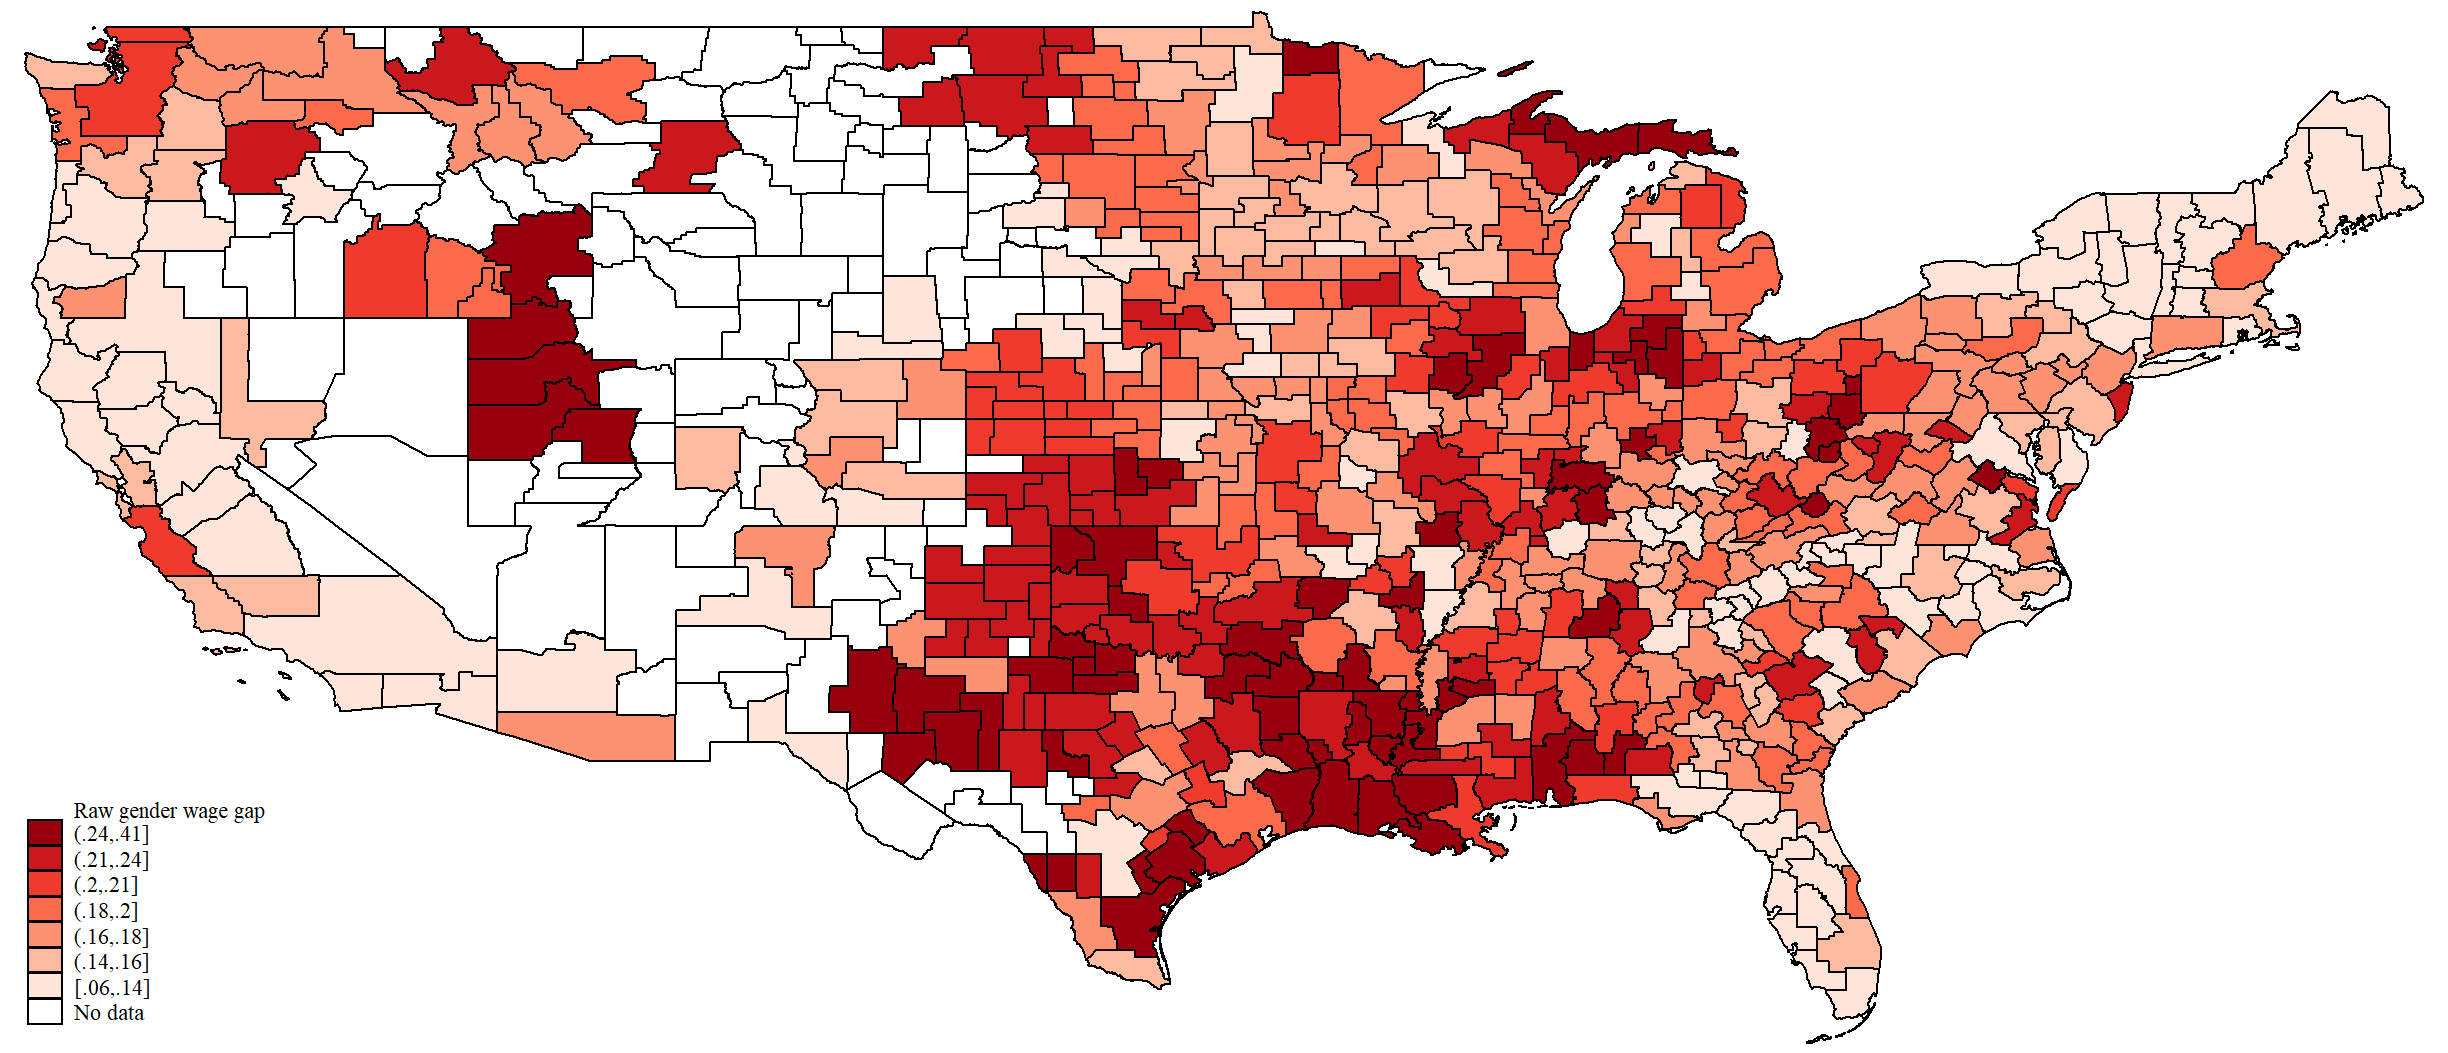
\includegraphics[width=1\textwidth]{../2_analysis/output/figures/raw_wage_map2020_full_time}
\par \begin{minipage}[h]{\textwidth}{\tiny\textbf{Note:} darker colors denote higher relative wages for men. Figure restricts to czones with population densities above 1 person per km$^2$ and full-time year-round workers.}\end{minipage}
\end{figure}

%\end{frame}

%\begin{frame}{Dispersion in the gap has remained over the whole period} 
%	\begin{figure}[!h]
\centering
\caption{Evolution of raw gender gap across CZ}
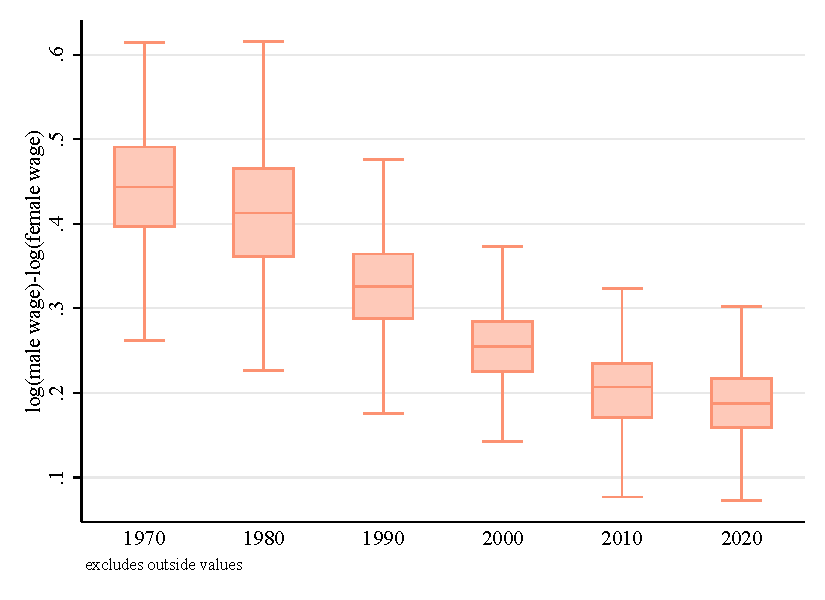
\includegraphics[width=.6\textwidth]{../2_analysis/output/figures/cz_gap_dispersion_full_time}
\par \begin{minipage}[h]{\textwidth}{\scriptsize\textbf{Note:} figure restricts to CZ with more than people per km$^2$ and full-time year-round workers..}\end{minipage}
\end{figure}

%\end{frame}

%\begin{frame}{Across CZ differences in the gap are persistent} 
%	I run the regression,
%	\beqns
%			w^{male}_{rt}-w^{female}_{rt}=\alpha_t+\beta_t(w^{male}_{r1970}-w^{female}_{r1970})
%	\eeqns
%	\begin{figure}[!h]
\centering
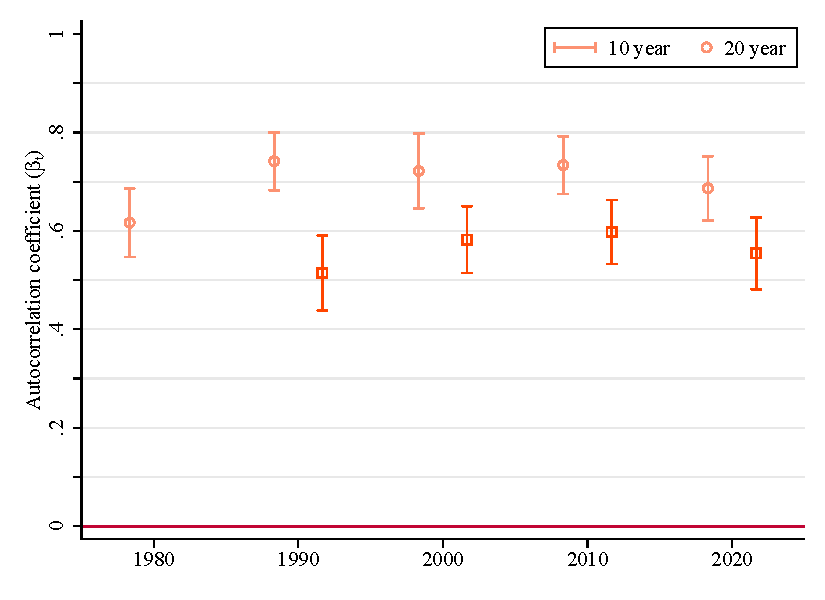
\includegraphics[width=.6\textwidth]{../2_analysis/output/figures/cz_gender_gap_persistence_full_time}
\par \begin{minipage}[h]{\textwidth}{\scriptsize\textbf{Note:} figure restricts to CZ with more than people per km$^2$ and full-time year-round workers.. Bars show 95\% robust confidence intervals. Standard errors are clustered at the CZ level. Dependent and independent variables are standardized}\end{minipage}
\end{figure}

%\end{frame}


\section{Basic regressions}

\begin{frame}{Accounting for individual characteristics}
\alert{\textbf{Route A}}: \newline
\begin{enumerate}
	\item Run on individual-level data:
	\beqns
		wage_{irt}^g=X_{iry}^g\gamma_t+\lambda_{rt}^g+\varepsilon_{irt}^g
	\eeqns
	\item In a second stage run:
	\beqns
		\hat{\lambda}_{rt}^{male}-\hat{\lambda}_{rt}^{female}=\tau_t+\beta_t\log(density)_{rt}+\varepsilon_{irt}^g
	\eeqns
\end{enumerate}
\end{frame}
\begin{frame}{Accounting for individual characteristics}
\alert{\textbf{Route B}}: \newline
If wages are determined at the individual level by the model:
\beqns
	w_{irt}^g=X_{irt}^g\gamma_t+\tau_tmale_i+\varepsilon_t
\eeqns
By aggregating at the CZ level this model becomes:
\beqns
w^{male}_{rt}-w^{female}_{rt}=\tau_t+ (\bar{X}_{rt}^{male}-\bar{X}_{rt}^{female})\gamma_t+u_t
\eeqns
Thus I run regressions of the form:
\beqns
w^{male}_{rt}-w^{female}_{rt}=\tau_t+ (\bar{X}_{rt}^{male}-\bar{X}_{rt}^{female})\gamma_t+\beta_t\log(density)_{rt}+u_t
\eeqns
\end{frame}
\begin{frame}{Route A}
\begin{figure}[!h]
\centering
\caption{Coefficient on population density $ \beta_t $ controlling for worker characteristics}
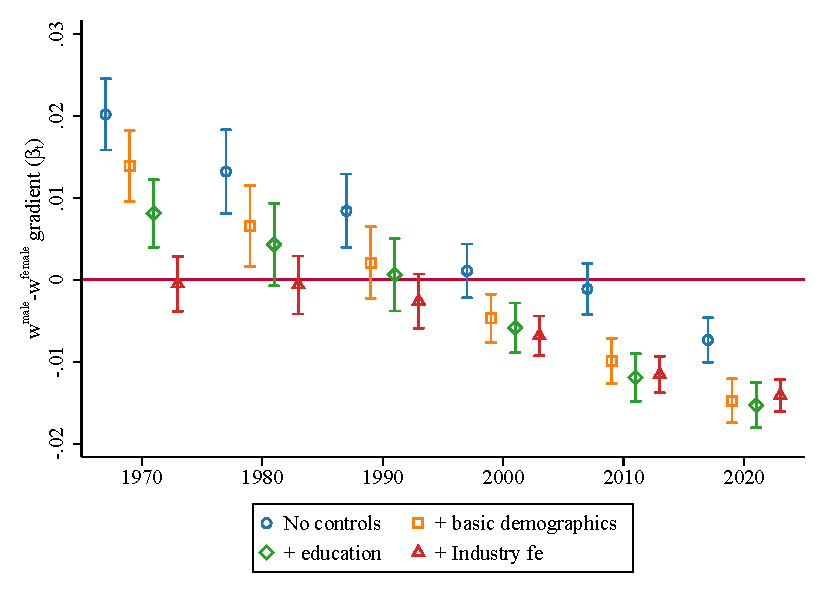
\includegraphics[width=.6\textwidth]{../2_analysis/output/figures/with_control_gradients_individual_l_czone_density_full_time}
\par \begin{minipage}[h]{\textwidth}{\tiny\textbf{Note:} figure restricts to CZ with more than 1 people per km$^2$. The regressions are done on data aggregated at the CZ level after residualizing individual-level characteristics. Bars show 95\% confidence intervals. Errors clustered at the CZ-level.}\end{minipage}
\end{figure}

\end{frame}
\begin{frame}{Route B}
\begin{figure}[!h]
\centering
\caption{Coefficient on population density $ \beta_t $ controlling for worker characteristics}
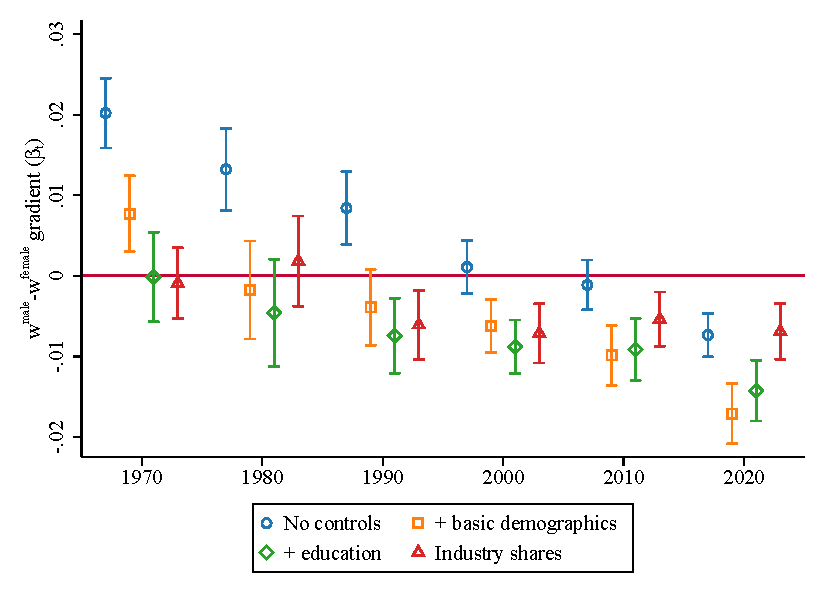
\includegraphics[width=.6\textwidth]{../2_analysis/output/figures/with_control_gradients_l_czone_density_full_time}
\par \begin{minipage}[h]{\textwidth}{\scriptsize\textbf{Note:} figure restricts to CZ with more than 1 people per km$^2$. The regressions are done on data aggregated at the CZ level. Bars show 95\% robust confidence intervals.}\end{minipage}
\end{figure}

\end{frame}



\end{document}

